\section{Introduction}
\label{sec:introduction}

Large Language Model (LLM) agents have shown strong capabilities in complex interactive tasks, including web navigation~\citep{yao2022webshop}, embodied household manipulation~\citep{shridhar2020alfworld}, and tool-augmented question answering~\citep{yao2022react}. 
Yet most agents treat task as episode~\citep{yao2022react, shinn2023reflexion}, struggling to learn from past successes or failures even when structurally similar problems have been encountered~\citep{xia2025skillrl}.
Since many tasks share recurring subproblems and compositional action patterns, an agent that can \emph{learn from experience}---extracting reusable knowledge from past interactions---would avoid redundant exploration, transfer strategies to similar tasks, and progressively build up the ability to solve more complex problems.

To reuse experience, a common approach is to maintain a \emph{skill library}, which stores reusable units of knowledge for solving recurring subproblems~\citep{wang2023voyager, zhao2024expel, xia2025skillrl}. 
A skill can be either manually designed by humans~\citep{xu2026agent} or automatically acquired from agent experience---for instance, by distilling successful trajectories into natural language~\citep{zhao2024expel, xia2025skillrl} or executable programs~\citep{wang2023voyager}. 
Compared with manually crafted skills, automatically acquired skills are more scalable and can continuously expand as the agent encounters new tasks and environments. 
Therefore, we focus on automatically acquiring skills from interaction trajectories.

Despite their promise, existing skill libraries are often organized as flat collections, where each skill is stored as an independent entry and retrieved mainly by semantic similarity~\citep{xia2025skillrl, zhao2024expel, liu2025simplemem}. 
This ignores the fact that skills are inherently related: some skills are prerequisites for others, some enhance others, and some frequently co-occur in successful trajectories. 
As a result, flat libraries suffer from two key limitations. 
First, \textbf{retrieval is not compositional}. 
Complex tasks often require an ordered sequence of skills; for example, a ``heat and place'' task in ALFWorld may require locating an object, picking it up, heating it with an appliance, and then placing it at the target destination. 
A flat Top-$K$ retriever can return relevant skills, but it does not indicate their dependencies or execution order. 
Second, \textbf{skill updates are not structured}. 
When skills are maintained independently, the library lacks explicit evidence for merging redundant skills, splitting overly broad skills, deprecating obsolete skills, or strengthening useful relations between skills~\citep{xu2026agent}.
These limitations suggest that the core problem is not only how to acquire skills, but also how to  \emph{organize, retrieve, and update} them. 
If inter-skill relations are explicitly represented, retrieval can produce dependency-aware skill sequences rather than unordered hints, and both individual skills and their relations can be updated in a principled way.

Motivated by this, we propose \textsc{SkillGraph}, a framework that organizes skills into a structured graph and co-evolves it with the agent's policy through reinforcement learning (RL). 
In \textsc{SkillGraph}, nodes represent skills distilled from trajectories, while typed edges capture relations such as prerequisite, enhancement, and co-occurrence. \textsc{SkillGraph} consists of three stages. 
First, \textbf{graph construction} builds an initial skill graph from interaction trajectories, making inter-skill relations explicit. 
Second, \textbf{graph-aware retrieval} starts from task-relevant seed skills, expands along graph edges, and orders retrieved skills according to their dependencies, producing a coherent skill sequence for decision-making. 
Third, \textbf{graph evolution} updates the graph during training by refining skill nodes and adjusting edge relations according to skill usage and success rate. 
Together, these stages form a closed loop: the skill graph provides structured guidance for policy learning, while the improving policy generates new trajectories that further refine the graph.

\begin{figure}[t]
    \centering
    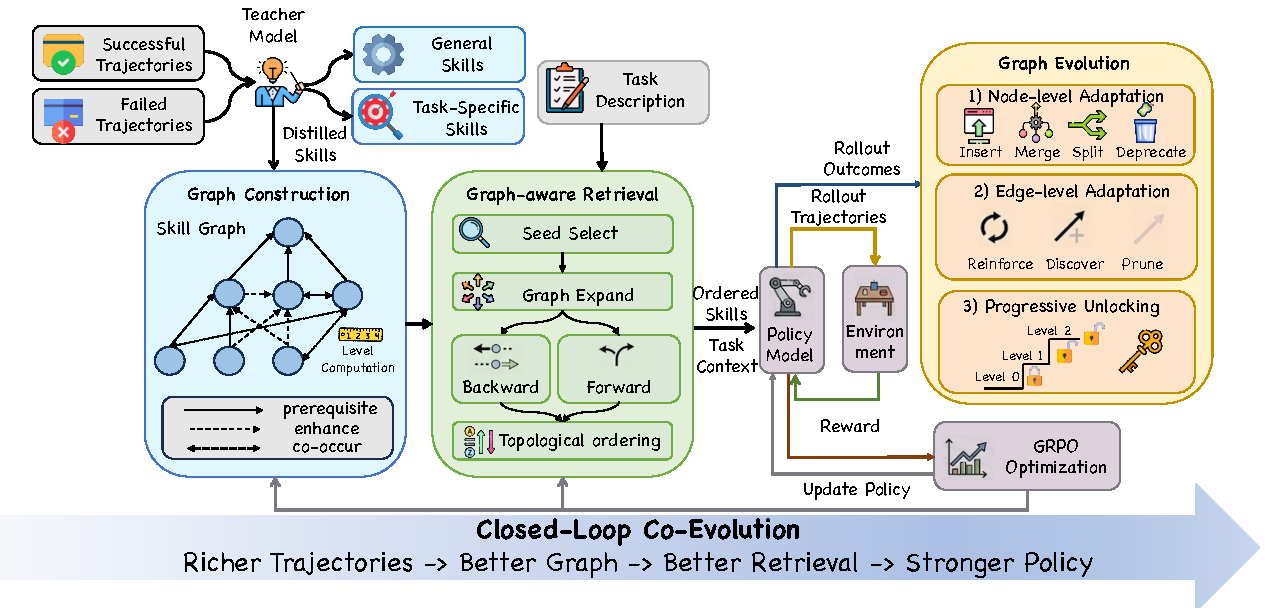
\includegraphics[width=\linewidth]{figure/overview.pdf}
    \vspace{-20pt}
    \caption{Overview of \textsc{SkillGraph}. The skill graph and the agent's policy \emph{co-evolve} through a closed loop: \textbf{(1)}~graph construction distills skills and their typed relations (prerequisite, enhancement, co-occurrence) from trajectories; \textbf{(2)}~graph-aware retrieval traverses these relations to produce dependency-ordered skill sequences that guide the policy; \textbf{(3)}~graph evolution uses training feedback to refine skill nodes, adjust edge weights, and restructure the graph, which in turn improves future retrieval and policy learning.}
    \label{fig:overview}
    \vspace{-20pt}
\end{figure}

Empirically, we evaluate \textsc{SkillGraph} on ALFWorld~\citep{shridhar2020alfworld}, WebShop~\citep{yao2022webshop}, and seven search-augmented question answering tasks~\citep{kwiatkowski2019nq}, covering embodied manipulation, web navigation, and information retrieval. 
Experimental results show that \textsc{SkillGraph} achieves state-of-the-art performance across benchmarks, with especially strong gains on complex multi-step tasks requiring skill composition. 
Further analysis shows that the graph structure improves skill reuse, reduces redundancy compared with flat libraries, and enables transfer of compositional knowledge from simpler tasks to more complex ones.

Our main contributions are summarized as follows:
\begin{itemize}[leftmargin=*, nosep]
    \item We propose a graph-structured formulation of skill library for LLM agents, where skills are connected by explicit prerequisite, enhancement, and co-occurrence relations.
    \item We introduce \textsc{SkillGraph}, a closed-loop framework that supports dependency-aware skill retrieval and structured skill updates during RL.
    \item We conduct experiments on ALFWorld, WebShop, and seven search-augmented QA tasks, demonstrating state-of-the-art performance and substantial gains on complex multi-step tasks.
\end{itemize}